% Bar Verteilung der Biogasaufbereitungsverfahren in Deutschland 2017

\begin{figure}[H]
	\centering
	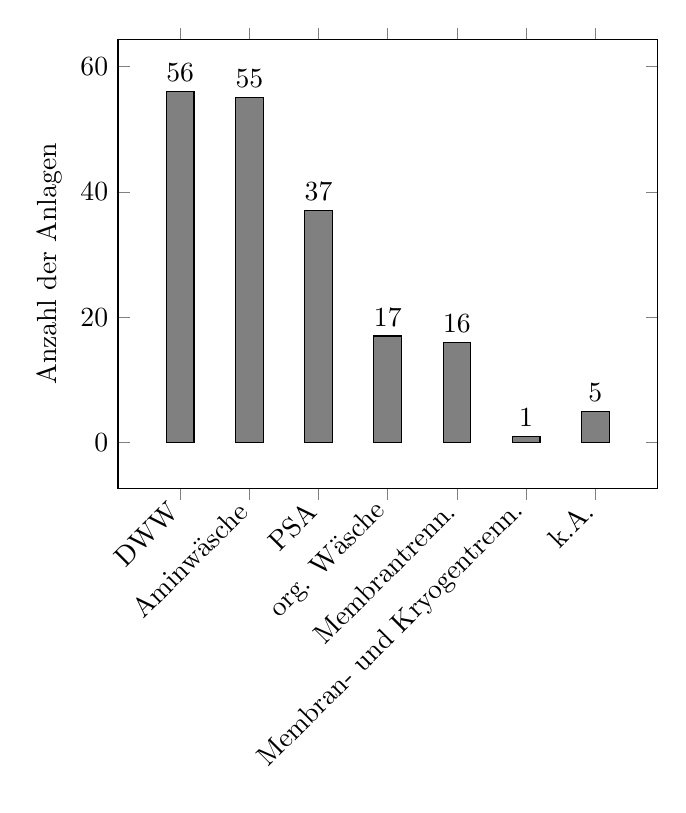
\begin{tikzpicture}
		\begin{axis}[
		ybar,
		enlargelimits=0.15,											% äüßerste bar plots nicht am Limit der x-Achse
		ylabel={Anzahl der Anlagen},
		symbolic x coords={DWW,
			Aminwäsche,
			PSA,
			org. Wäsche,
			Membrantrenn.,
			Membran- und Kryogentrenn.,
			k.A. 
		},
		xtick=data,
		nodes near coords,											% Zahlen auf den bar plots
		nodes near coords align={vertical},
		nodes near coords style={/pgf/number format/.cd,fixed,fixed zerofill,precision=0},
		x tick label style={rotate=45,anchor=east},
		]
		\addplot[black,fill=black!50!white] coordinates {
			(DWW,56) (Aminwäsche,55) (PSA,37) (org. Wäsche,17) (Membrantrenn.,16) (Membran- und  Kryogentrenn.,1) (k.A.,5)
		};
		\end{axis}
	\end{tikzpicture}
	\caption{Verteilung der in Deutschland eingesetzten Verfahren zur Biogasaufbereitung zu Biomethan \parencite{Grom17}; \textit{Eigene Darstellung}}
	\label{fig:gas-upgradingDE}
\end{figure}


